\documentclass[12pt,a4paper]{article}
\usepackage[utf8]{inputenc}
\usepackage[spanish]{babel}
\usepackage{amsmath}
\usepackage{amsfonts}
\usepackage{amssymb}
\usepackage{makeidx}
\usepackage{hyperref}
\usepackage{graphicx}
\usepackage[left=2cm,right=2cm,top=2cm,bottom=2cm]{geometry}
\graphicspath{ {./images/} }

\title{Gymodo}
\begin{document}

\begin{titlepage}
    \begin{center}
        \vspace*{1cm}
            
        \Huge
        \textbf{Gymodo}
            
        \vspace{0.5cm}
        \LARGE
        La mejor App para tu gym.
        
        \vfill
        

        Edgar Luque, Shah Sawar, Ronald Intriago\\
            
        \vspace{0.8cm}
           
            
        \Large
        Desarrollo de Aplicaciones Multiplataforma\\
        Escola del Treball\\
        Barcelona\\
        \today
            
    \end{center}
\end{titlepage}

\newpage

\begin{abstract}
Gyomodo es una aplicación que tiene como objetivo resolver los problemas que puedan tener los gymnasios en estos tiempos modernos, pero sobretodo, problemas originados a partir de la pandemia del Covid-19.

Este documento explica el desarrollo de esta aplicación, su funcionalidad y la organización del equipo.
\end{abstract}

\newpage

\tableofcontents

\newpage

\section{Análisis funcional}

\subsection{Tecnología usada}

\begin{itemize}
\item Git
\item Asana
\item toggl
\item Android Studio
\end{itemize}

\newpage

\subsection{Diagrama UML}

\begin{figure}[h]
 	\centering
	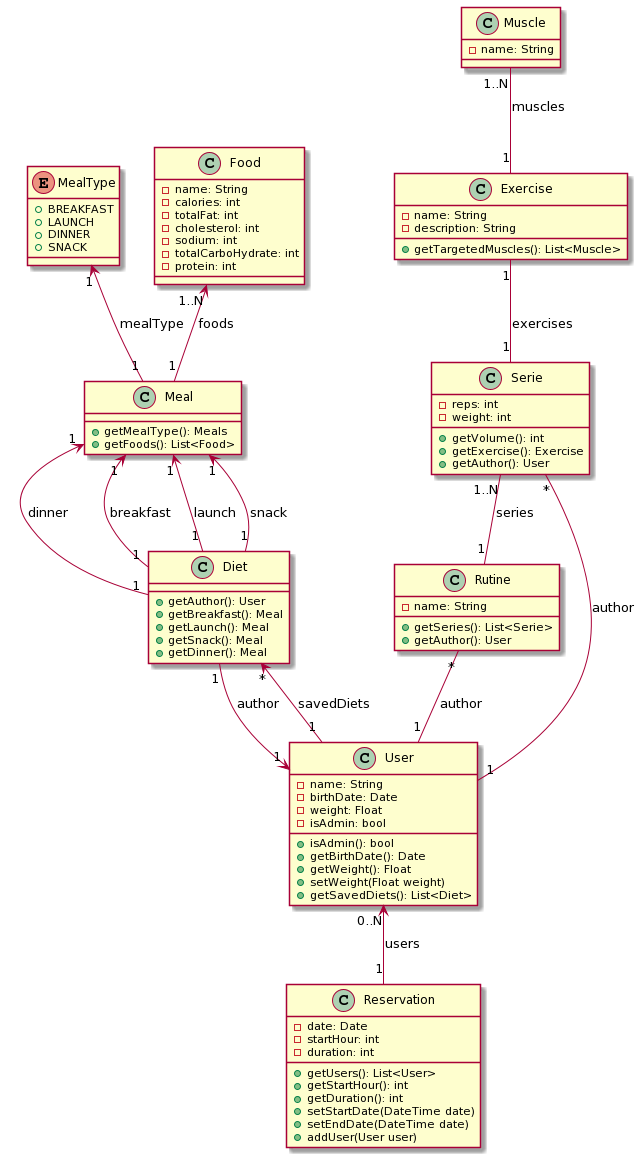
\includegraphics[width=0.6\textwidth]{uml}
	\caption{Diagrama UML}
\end{figure}

\newpage

\subsection{Diagrama Casos de Uso}

\begin{figure}[h]
 	\centering
	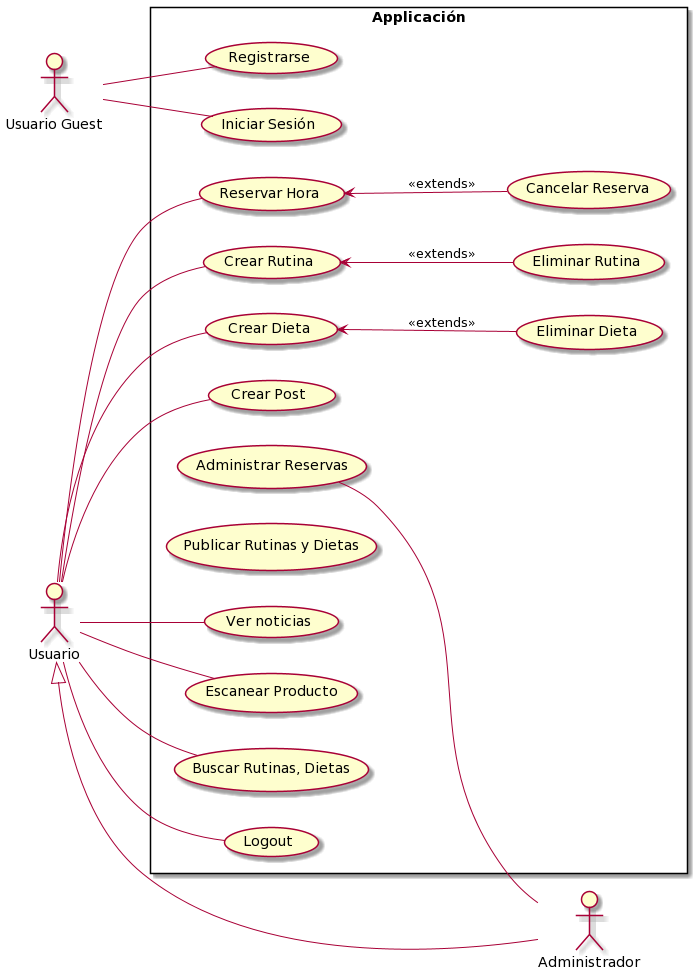
\includegraphics[width=0.6\textwidth]{casos_uso}
	\caption{Diagrama de Casos de Uso}
\end{figure}

\newpage

\subsection{Diagrama Relacional (bases de datos)}

\begin{figure}[h]
 	\centering
	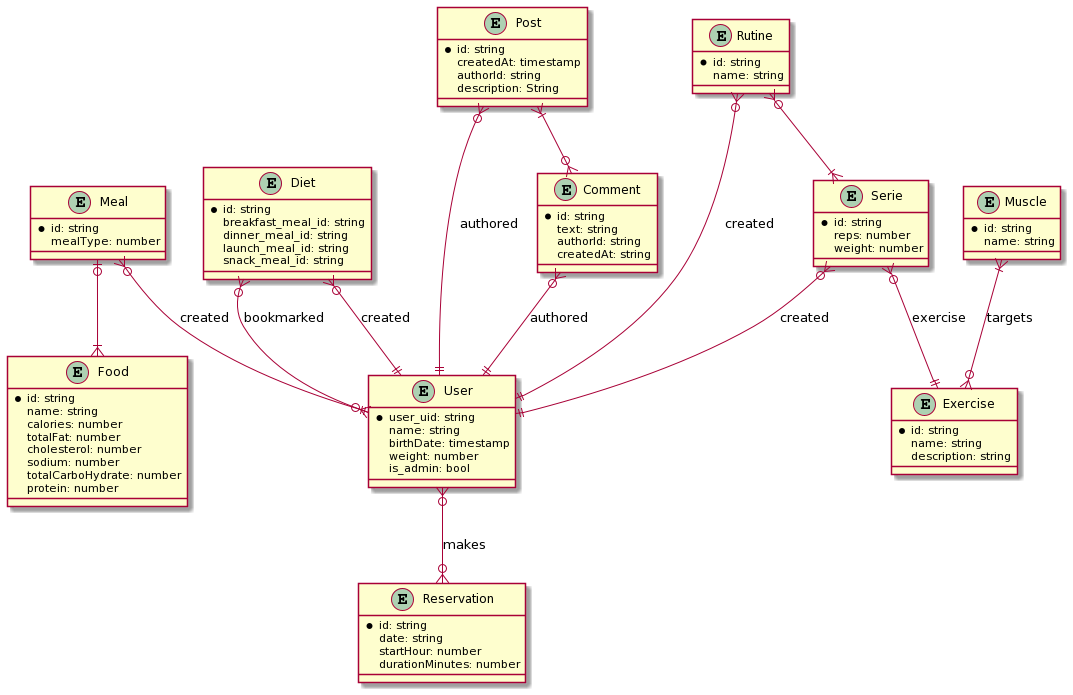
\includegraphics[width=0.6\textwidth]{diagramaer}
	\caption{Diagrama Entidad Relacion}
\end{figure}

\newpage

\subsection{Mockup}
\href{https://mockittapp.wondershare.com/app/3398ef738f7ac4f35fae5df4eb77004473612d19?simulator_type=device&sticky}{Link al mockup}

\end{document}